\chapter{Escopo do Projeto}
A proposta de projeto é uma aplicação \textit{web} voltada para auxiliar no acompanhamento da evolução no rendimento dos alunos nas atividades escolares.

\section{Histórias de Usuário}
Para o projeto, foram escolhidas as histórias de usuário para estabelecer as necessidades do sistema. 

\subsection{Cadastros}
Eu, como administrador, quero criar outro administrador, para que alguém possa me ajudar nas tarefas administrativas do sistema

Eu, como administrador, gostaria de cadastrar escolas para meus clientes.

Eu, como administrador, gostaria que, ao criar uma escola, fosse enviado um e-mail para o gestor com uma página para que ele complemente as informações da escola e do seu usuário.

Eu, como administrador, quero visualizar um resumo do uso do sistema, para que eu possa tomar decisões com base no uso.

\subsection{Acessos e Logins}

Eu, como usuário do sistema, gostaria de poder definir a minha senha durante o primeiro acesso a aplicação para garantir a segurança do acesso.

Eu, como usuário do sistema, gostaria de fazer o login na aplicação para garantir a privacidade dos meus dados.

Eu, como usuário do sistema, gostaria de poder recuperar minha senha.

Eu, como administrador, quero revogar os acessos de outro administrador, para caso ele seja demitido da empresa.

Eu, como administrador, quero revogar os acessos de um gestor e sua escola, para caso eles criem conteúdos inadequados.

Eu, como administrador, quero desativar a escola, para suspender o uso de seus usuários quando os mesmos estiverem em débito com a empresa.

\subsection{Parametrização de turmas}

Eu, como gestor, gostaria de cadastrar uma nova turma para os alunos do próximo ano letivo.

Eu, como gestor, gostaria de dar o cargo de professor a um novo usuário caso um novo professor seja contratado.

Eu, como gestor, gostaria de atribuir professores e alunos as suas devidas disciplinas para facilitar a interação entre ambos os lados.

Eu, como gestor, gostaria de atribuir dois professores em uma mesma disciplina para uma turma de alunos que pode ser dividida.

\subsection{Painel de turmas}
Eu, como gestor, gostaria de visualizar todas as turmas e disciplinas cadastradas para uma melhor administração das mesmas.

Eu como professor, gostaria de visualizar as turmas atribuídas a mim para postar meus conteúdos por turma.

\subsection{Atividades}
Eu, como professor, gostaria de cadastrar atividades no sistema para que meus alunos façam.

Eu, como professor, gostaria de marcar se uma atividade é avaliativa ou não e se é entregável ou não para poder atribuir melhor as conquistas.

Eu, como aluno, gostaria de ter fácil acesso às minhas atividades, para não perder tempo procurando-as.

Eu, como aluno, gostaria de poder visualizar as minhas atividades ordenadas por data de vencimento, para não perder nenhum prazo de entrega.

Eu, como aluno, gostaria de visualizar todos os detalhes da atividade para não ter dúvidas sobre como realizá-la.

Eu, como professor, gostaria de receber as atividades no sistema para poder corrigi-las.

Eu, como professor, gostaria de atribuir feedback aos meus alunos das atividades para que possa retornar uma nota caso for avaliativa.

Eu, como aluno, gostaria de ver o feedback das correções das atividades que valem nota, para saber o que preciso melhorar.

\subsection{Conquistas}

Eu, como gestor, gostaria de cadastrar diferentes tipos de conquistas para que os alunos possam alcançá-las.

Eu, como aluno, gostaria de visualizar minhas conquistas pendentes, para que eu corra atrás de conquistá-las e subir no ranking.

\subsection{Ranking}

Eu, como aluno mais inteligente da sala, gostaria de poder visualizar minha posição no ranking geral da turma, para alimentar meu ego.

Eu, como aluno, gostaria de poder visualizar minha posição no ranking por disciplina, para saber a disciplina que eu preciso me esforçar mais.

Eu, como aluno não tão bem empenhado, não gostaria que minha posição no ranking seja visível para outros alunos, a não ser que eu esteja entre os primeiros da minha liga, para não sofrer bullying.

Eu, enquanto aluno, gostaria de ver minha pontuação geral, e a pontuação dos três primeiros do ranking da minha liga, para saber o quanto eu preciso me esforçar para alcançá-los.
 
Eu, como professor, gostaria de ver o ranking de cada turma para poder fazer o acompanhamento da mesma.

Eu como aluno, gostaria de saber quais as conquistas/pontuações mínimas eu preciso ter para avançar para próxima liga.

Eu, como gestor, gostaria de ver o ranking de cada turma para poder fazer o acompanhamento das mesmas.

\subsection{Dashboards}

Eu, como gestor, gostaria de ver o desempenho de cada turma e de alunos em particular para poder acompanhar cada caso com a devida atenção necessária.


\section{Funcionalidades}
Considerando as histórias de usuário mapeadas, a aplicação contará com o módulo de cadastros que permitirá que o usuário (coordenador, diretor ou pedagogo) realize o cadastro de turmas, disciplinas, gestores e alunos.


Além da configuração básica, o gestor poderá atribuir os professores e alunos às turmas e disciplinas previamente cadastradas. Ademais, deverá configurar a estrutura de conquistas e os parâmetros para que sejam alcançados pelos alunos.


Ao acessar a aplicação, o professor poderá visualizar as turmas e disciplinas atribuídas a ele. Para cada turma/disciplina ele poderá visualizar o ranking dos alunos, inserir e receber as atividades deles.


Quando o aluno acessar a aplicação, o mesmo poderá visualizar as atividades pendentes e o painel de conquistas que apresentará as conquistas alcançadas e não alcançadas por ele. Ademais, poderá visualizar o ranking da turma, sua posição em relação aos seus amigos e a pontuação necessária para que ele suba para a liga (\textit{\glspl{tier}}) imediatamente mais alta.


A aplicação também fornecerá um \textit{\gls{dashboard}} que conterá gráficos com visões gerenciais que indicam o desempenho por turma e por aluno. Esse \textit{\gls{dashboard}} estará disponível apenas para  usuários com o perfil gestor.
As funcionalidades a serem implementadas estão descritas com mais detalhes nos subcapítulos a seguir. 


\subsection{Login e perfis}
O módulo de acesso permitirá que usuários cadastrados acessem o sistema; todos os processos relacionados à definição e reinicialização de senha estão contemplados neste módulo. Também será possível definir, para um determinado perfil, quais são as suas permissões de acesso.
Inicialmente, contempla-se nesta proposta quatro categorias de perfil de acesso: 


\begin{itemize}
\item \textbf{Perfil aluno}: poderá acessar as disciplinas referentes à turma que ele foi inserido, painel de atividades, painel de conquistas, sua posição no ranking e os alunos que ocupam os três primeiros lugares de cada liga (\textit{\glspl{tier}}). A Figura 3 exibe um \textit{\gls{wireframe}} da tela para o perfil do aluno.

\begin{figure}[htb]
    \centering
	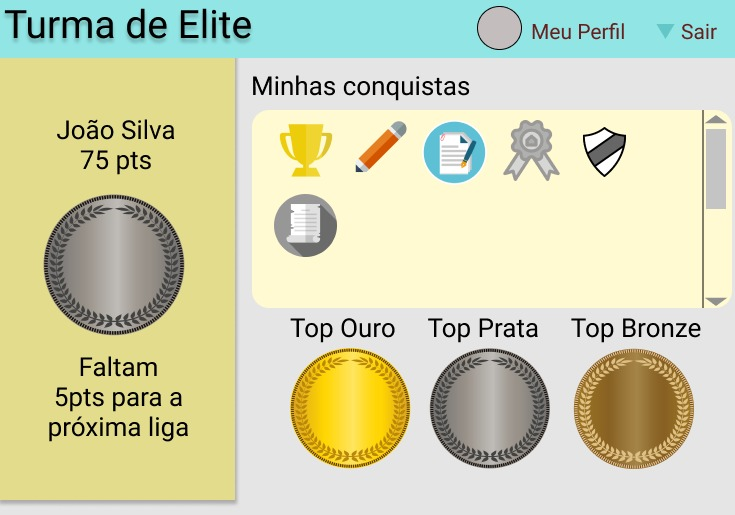
\includegraphics[width=11cm]{imagens/tela-aluno-2.jpeg}
	\caption{\textit{\gls{wireframe}} da tela do aluno}
	\fonte{Os autores}
\end{figure}
\FloatBarrier

\item \textbf{Perfil professor}: poderá visualizar as turmas atribuídas a ele e o ranking da turma. Será responsável por postar as atividades e ao corrigi-las, atribuir a pontuação para os alunos. A Figura 4 exibe um \textit{\gls{wireframe}} da tela para o perfil do professor.

\begin{figure}[htb]
    \centering
	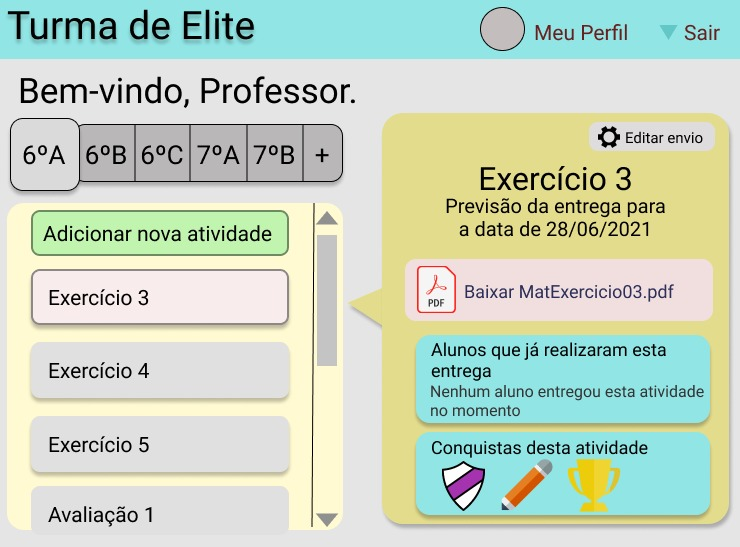
\includegraphics[width=11cm]{imagens/tela-professor.jpeg}
	\caption{\textit{\gls{wireframe}} da tela do professor}
	\fonte{Os autores}
\end{figure}
\FloatBarrier

\item \textbf{Perfil gestor}: poderá visualizar todas as turmas cadastradas, o ranking de cada uma delas e o \textit{\gls{dashboard}}. Será responsável por realizar os cadastros e parametrizações do sistema. A Figura 5 exibe um \textit{\gls{wireframe}} da tela para o perfil do gestor.

\begin{figure}[htb]
    \centering
	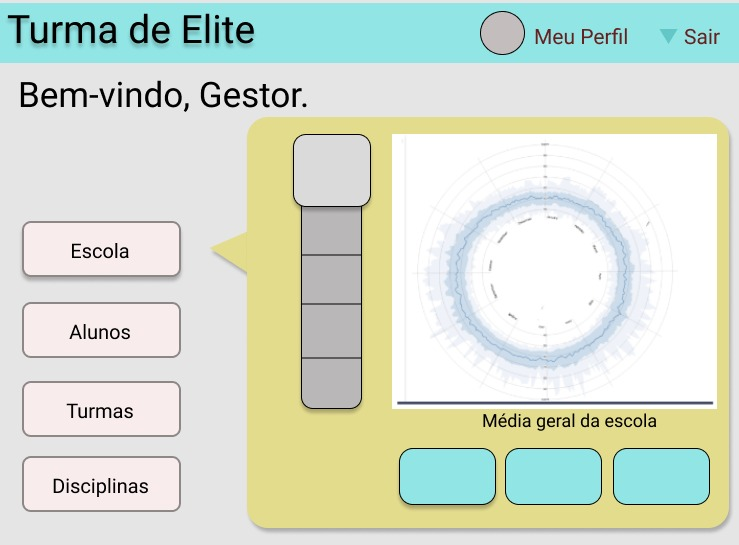
\includegraphics[width=11cm]{imagens/tela-gestor.jpeg}
	\caption{\textit{\gls{wireframe}} da tela do gestor}
	\fonte{Os autores}
\end{figure}
\FloatBarrier

\item \textbf{Perfil administrador}: Superusuário do sistema, será responsável pelo cadastro das escolas e seus respectivos gestores.
\end{itemize}


\subsection{Cadastros/Dados mestres}
Segundo os objetivos do projeto, são listados abaixo os cadastros básicos, essenciais ao funcionamento do sistema em questão. Para cada cadastro, o sistema deve permitir a inserção, listagem, alteração e exclusão (ou inativação) de registros. 
\begin{itemize}
\item \textbf{Usuários}: contempla os dados dos usuários que acessarão o sistema (gestores, professores e alunos).
\item \textbf{Turmas/disciplinas}: contempla os dados das turmas/disciplinas da escola;
\item \textbf{Conquistas}: contempla os dados das conquistas. Ao cadastrar uma conquista, o gestor deverá definir a recompensa pela sua conquista, o seu nível e os critérios para alcançá-la.
\item \textbf{Atividades}: contempla os dados das atividades. Uma atividade poderá gerar um entregável ou não.
\item \textbf{Escolas}: contempla os dados das escolas clientes da aplicação.
\end{itemize}


\subsection{Parametrização de turmas}
O gestor deverá utilizar esta funcionalidade para atribuir a cada turma, o professor responsável e os alunos. Para cada turma poderá ser atribuído um único professor. No caso de uma disciplina compartilhar mais de um professor, o gestor deverá criar uma disciplina para a mesma turma para cada professor e dividir os alunos entre elas. 

\subsection{Painel de turmas/disciplinas}
Este painel será exibido assim que o usuário acessar aplicação. Ele consiste em uma grade de botões que darão acesso ao ambiente da disciplina. Este painel estará disponível para as três visões previstas neste projeto, porém as turmas a serem listadas serão restringidas da seguinte forma:

\begin{itemize}
\item \textbf{Visão do aluno}: listará somente as disciplinas da turma no qual foi inserido.
\item \textbf{Visão do professor}: listará somente as turmas/disciplinas atribuídas a ele.
\item \textbf{Visão do gestor}: listará todas as turmas/disciplinas cadastradas.
\end{itemize}


\subsection{Módulo de atividades}
Este módulo será disponibilizado no ambiente da disciplina e será utilizado por professores e alunos. Através dele, o professor poderá postar as atividades e atribuir notas. Ao postar uma atividade o professor poderá informar a pontuação e o prazo de entrega. Caso a atividade possua um entregável, o professor deverá indicar também no momento do cadastro.


Para os alunos, ao acessar esta seção, eles poderão visualizar as atividades postadas pelo professor. Ao realizar uma atividade que necessita de um entregável, o aluno deverá realizar o \textit{upload} de um arquivo no formato especificado pelo professor na descrição da atividade, após a confirmação da entrega atividade ganhará um status “Pendente de avaliação”. Somente após a avaliação do professor, a atividade será marcada como concluída.


As atividades criadas que não geram entregáveis estão ligadas ao ensino presencial, na qual, ao passar uma atividade na sala, ou um dever de casa, o aluno mostrará a apostila para o professor, e ele dará o seu “visto” pela aplicação. 

\subsection{Painel de conquistas}
O painel de conquista estará disponível para o aluno. Cada aluno terá seu próprio painel de conquistas, e nele o aluno poderá visualizar as conquistas atingidas, as pendentes e as bloqueadas. 


O aluno poderá alcançar somente as conquistas atreladas a liga que ele se encontra e as imediatamente abaixo. A cada liga, as conquistas ficam mais difíceis de alcançar, porém as recompensas serão maiores. 
\subsection{Ranking de alunos por liga}
O sistema de ranqueamento do sistema Turma de Elite contemplará três ligas, sendo elas: bronze, prata e ouro. Cada liga conterá um ranking disponibilizado em duas visões (\textit{\gls{ranking}} por disciplina e \textit{\gls{ranking}} geral). Sempre ao final de um período pré-determinado, os três primeiros colocados de um ranking que possuem a pontuação mínima requerida pela liga superior, ganham um lugar na próxima liga, enquanto os três últimos descem para uma liga inferior.


Assim como o painel de turmas/disciplina, os \textit{\glspl{ranking}} estarão disponíveis para todos os usuários, porém de forma restringida dependendo do perfil.
\begin{itemize}
\item \textbf{Visão do aluno}: visualizará apenas os \glspl{ranking} referente à turma no qual o aluno está inserido. Em cada ranking o aluno saberá apenas o nome dos três primeiros colocados de cada liga e a sua posição caso ele não esteja entre os primeiros.
\item \textbf{Visão do professor}: visualizará os \glspl{ranking} das turmas atribuídas a ele. Em cada ranking, o professor poderá ver todos os alunos e suas respectivas posições.
\item \textbf{Visão do gestor}: visualizará os rankings de todas as turmas ativas na aplicação. Em cada \gls{ranking}, o gestor poderá ver todos os alunos e suas respectivas posições.
\end{itemize}

\subsection{Dashboard}
A aplicação também disponibilizará relatórios gerenciais para o perfil gestor como: histórico de desempenho por turma e por aluno.

%\section{Entrega Final}

%\itemPara a entrega completa do sistema Turma de Elite já está previsto, além de melhorias, %desenvolvimento de novas funcionalidades que %serão elencadas nos tópicos a seguir:
%\begin{itemize}
%\item  Criação do novo perfil "Pais e %responsáveis": melhoria no módulo de acesso, %o novo perfil permitirá que os pais ou %responsáveis pelo aluno acompanhe as %atividades do aluno.
%\item  Boletins: nova funcionalidade que %permitirá que os professores insiram as notas %das provas ao fim de cada bimestre.
%\item  Plano de aulas: nova funcionalidade %que permitirá que o professor realize seu %planejamento de aulas. Este plano de aulas %poderá ser convertido para um relatório que %estará disponível para download para os %gestores da escola;
%\item  Atividades programadas: melhoria que %permitirá que os professores programem a %postagem de atividades para seus alunos.
%\item  Notificações e Lembretes: melhoria que %permitirá que os usuários sejam notificados %por e-mail a respeito de ações tomadas na %aplicação como, por exemplo, confirmação de %envio de atividade.
%\end{itemize}



\section{\textit{Product Backlog}}
Com as histórias de usuário definidas, foi montado o \textit{Product Backlog} para definir a ordem de importância delas. A Figura 6 representa o resultado da priorização, segundo cada funcionalidade.  

\begin{figure}[htb]
    \centering
	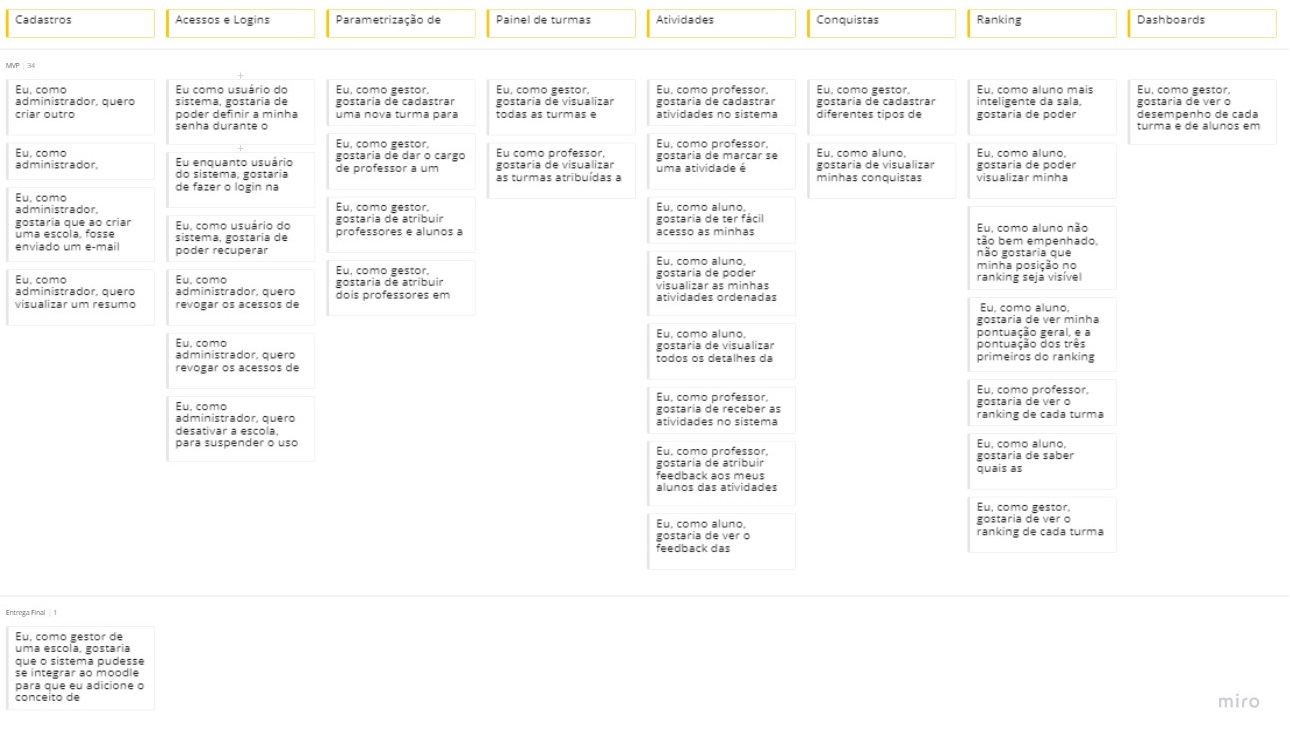
\includegraphics[width=16cm]{imagens/ProductBacklog.jpg}
	\caption{Product Backlog do Projeto Turma de Elite}
	\fonte{Os autores}
\end{figure}
\FloatBarrier

\section{MER e DER}
Para a modelagem de dados do projeto, foi elaborado o modelo entidade-relacionamento (MER) e, para representá-lo, foi feito o diagrama entidade-relacionamento (DER), conforme demostra a Figura 7.

\begin{figure}[htb]
    \centering
	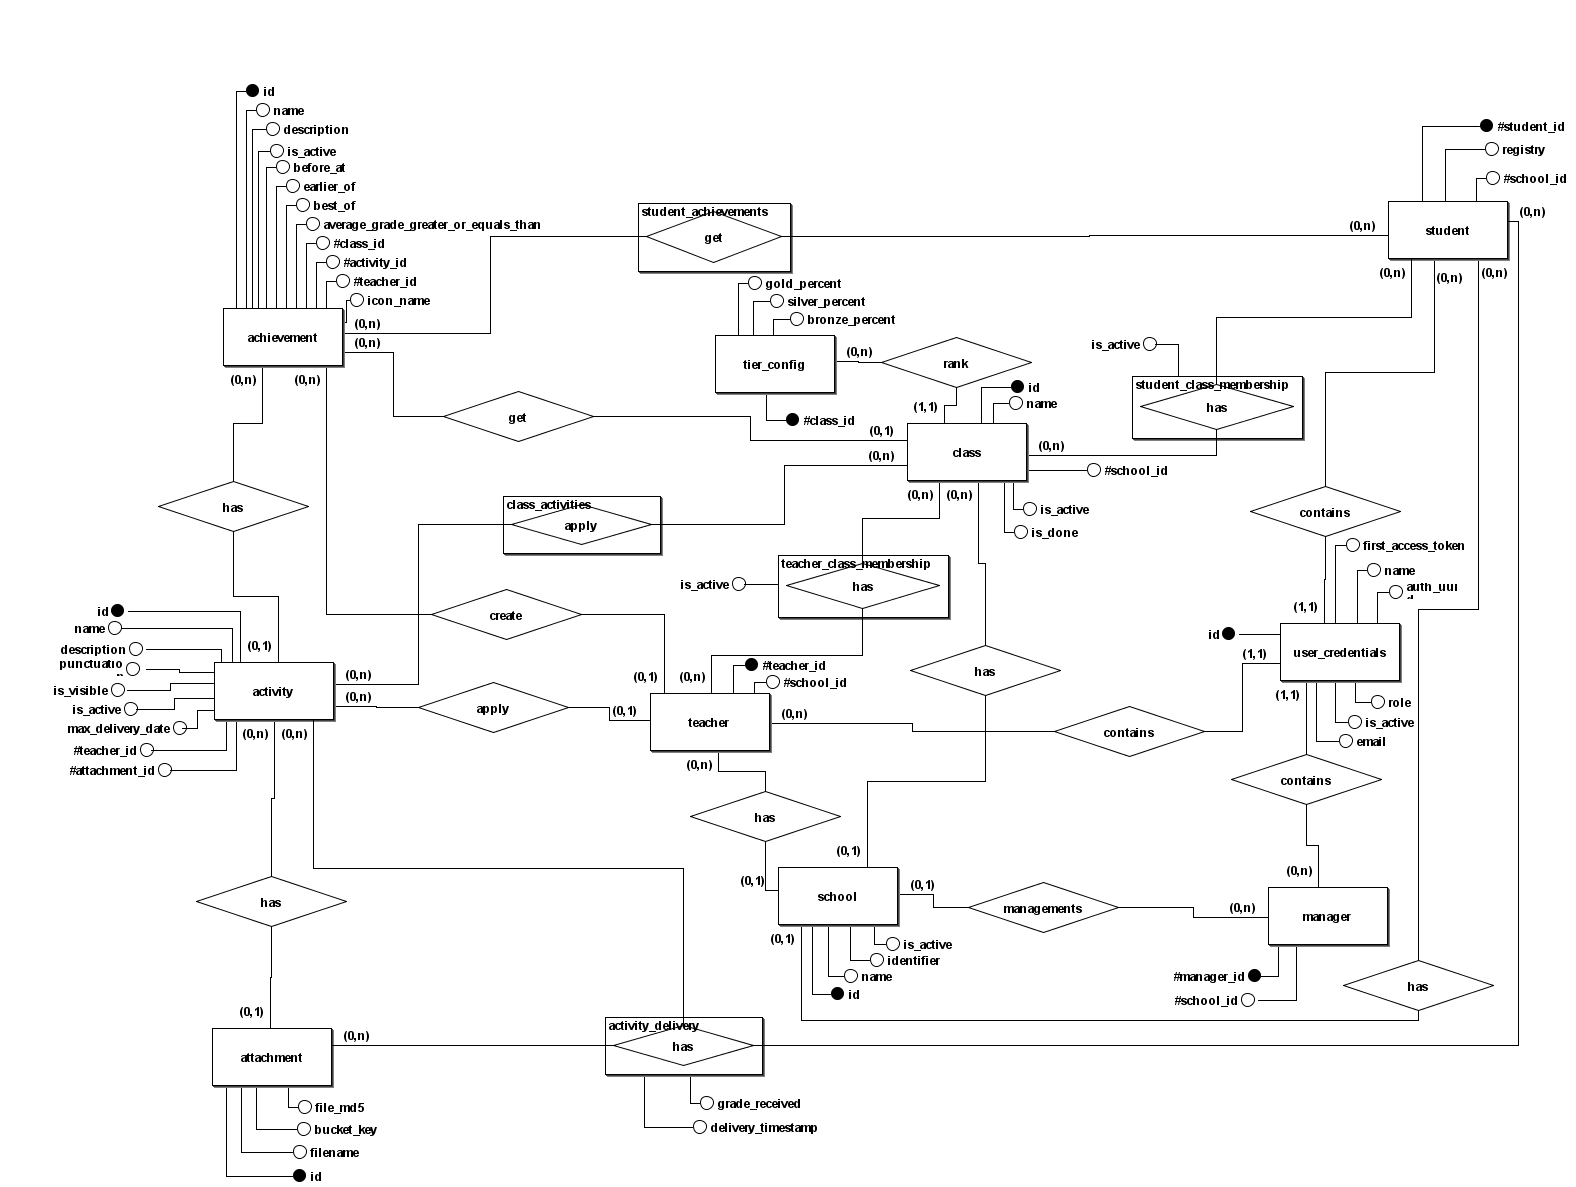
\includegraphics[width=16cm]{imagens/ModeloConceitual.png}
	\caption{Modelo Conceitual do Projeto Turma de Elite}
	\fonte{Os autores}
\end{figure}
\FloatBarrier


\section{Modelo Lógico}
Com o MER e DER mapeados, foi possível desenvolver o modelo lógico da aplicação, conforme mostra a figura 8.

\begin{figure}[htb]
    \centering
	\includegraphics[width=16cm]{imagens/ModeloLogico.png}
	\caption{Modelo Lógico do Projeto Turma de Elite}
	\fonte{Os autores}
\end{figure}
\FloatBarrier
